\documentclass{article}

\usepackage{amsmath}
\usepackage{mathtools}
\usepackage{amsfonts}
\usepackage{url}
\usepackage{xspace}
\usepackage{siunitx}
\usepackage{cancel}
\usepackage[usenames,dvipsnames]{xcolor}
\usepackage{tikz}
\usepackage{float}
\usepackage{booktabs}

\graphicspath{{./images/}}

\usepackage{vletters}
%\usepackage{simplewick}
\usepackage{wick}

\usepackage{enumitem}
\setlist[enumerate]{label=(\alph*)}

% Formatting options 
\frenchspacing
% \setlength{\parindent}{0 ex}
% \setlength{\parskip}{3 ex plus 2 ex minus 1 ex}

% Defined macros

\DeclareMathOperator{\csch}{csch}
\DeclareMathOperator{\sech}{sech}
\DeclareMathOperator{\perm}{\mathit{\hat{P}}}

\newcommand{\degree}[0]{\ensuremath{^\circ}\xspace}
\renewcommand{\implies}{\Rightarrow}
\newcommand{\eval}[1]{\ensuremath{\left<#1\right>}}
\newcommand{\ket}[1]{\ensuremath{\left| #1 \right>}}
\newcommand{\bra}[1]{\ensuremath{\left< #1 \right|}}
\newcommand{\mel}[3]{\ensuremath{\left<#1 \right|\! #2 \!\left| #3 \right>}}
\newcommand{\proj}[2]{\ensuremath{\left<#1 \middle| #2 \right>}}

\newcommand{\pmat}[1]{\ensuremath{\begin{pmatrix}#1\end{pmatrix}}}

\newcommand{\su}[0]{\ensuremath{\uparrow}}
\newcommand{\sd}[0]{\ensuremath{\downarrow}}

\newcommand{\pder}[2]{\ensuremath{\frac{\partial #1}{\partial #2}}}
\newcommand{\ppder}[2]{\ensuremath{\frac{\partial^2 #1}{\partial #2^2}}}
\newcommand{\ppmder}[3]{\ensuremath{\frac{\partial^2 #1}{\partial #2 \partial #3}}}

\newcommand{\pderc}[3]{\ensuremath{\left( \frac{\partial #1}{\partial #2} \right)_{\!\!#3}}}
\newcommand{\ppmderc}[4]{\ensuremath{\left( \frac{\partial^2 #1}{\partial #2 \partial #3} \right)_{\!\!#4}}}

\newcommand{\phias}[0]{\ensuremath{\Phi^\text{AS}}}
\newcommand{\phisub}[2]{\ensuremath{\phi_{#1}\!\left(#2\right)}}
\newcommand{\psisub}[2]{\ensuremath{\psi_{#1}\!\left(#2\right)}}
\newcommand{\phisubs}[2]{\ensuremath{\phi^*_{#1}\!\left(#2\right)}}
\newcommand{\psisubs}[2]{\ensuremath{\psi^*_{#1}\!\left(#2\right)}}

\newcommand{\ah}[1]{\ensuremath{a_{#1}}}
\newcommand{\ad}[1]{\ensuremath{a^{\dagger}_{#1}}}

% Titles and headers

\title{Phy 981 Project}
\author{Josh Bradt}
\date{March 9, 2015}

\makeatletter
\let\thetitle\@title
\let\theauthor\@author
\makeatother

\usepackage{fancyhdr}
\pagestyle{fancy}
\chead{\footnotesize \MakeUppercase{\thetitle}} \rhead{\footnotesize\thepage}
\cfoot{}
\renewcommand{\headrulewidth}{0pt}

% Setion numbering
\renewcommand{\thesection}{\alph{section})}

\begin{document}

\maketitle

\section{Commutators and operators}
	
	The Hamiltonian used in the problem is given as
	\begin{equation*}
		\hat H = \hat H_0 + \hat V
	\end{equation*}
	where
	\begin{equation}
		\hat H_0 = \xi \sum_{p\sigma} (p-1) a_{p\sigma}^\dagger a_{p\sigma}
	\end{equation}
	and the matrix element of the potential is
	\begin{equation}
		\mel{q+q-}{V}{s+s-} = -g.  \label{eq:potelmnt}
	\end{equation}
	The form of this matrix element implies that the two-body part of the Hamiltonian can be written in an anti-symmetric form as
	\begin{equation}
		\hat V = -g \sum_{pq} a^\dagger_{p+} a^\dagger_{p-} a_{q-} a_{q+}.
	\end{equation}

	Both parts of the Hamiltonian commute with the spin projection operator
	\begin{equation*}
		\hat S_z = \frac{1}{2} \sum_{p\sigma} \sigma a^\dagger_{p\sigma} a_{p\sigma}.
	\end{equation*}
	For the unperturbed part, the commutator can be written down as
	\begin{equation}
		\left[\hat H_0, \hat S_z \right] = \frac{\xi}{2} \left[ \sum_{p\sigma} (p-1) a_{p\sigma}^\dagger a_{p\sigma}, \sum_{p\sigma} \sigma a^\dagger_{p\sigma} a_{p\sigma} \right]. \label{eq:comm1}
	\end{equation}
	Recall, however, that the creation and annihilation operators anticommute. Thus, this commutator boils down to whether
	\begin{equation}
		a^\dagger_{p\sigma} a_{p\sigma} a^\dagger_{p'\sigma'} a_{p'\sigma'} \stackrel{?}{=} a^\dagger_{p'\sigma'} a_{p'\sigma'} a^\dagger_{p\sigma} a_{p\sigma}. \label{eq:comm1ops}
	\end{equation}
	Since the operators are paired together, it will take an even number of permutations to make the right-hand side of (\ref{eq:comm1ops}) look like the left-hand side. Therefore, the two sides are equal, and the commutator (\ref{eq:comm1}) is zero.

	The commutator between the potential and the spin projection operator is
	\begin{equation*}
		\left[ \hat V, \hat S_z \right] = -\frac{g}{2} \left[ \sum_{pq} a^\dagger_{p+} a^\dagger_{p-} a_{q-} a_{q+}, \sum_{p\sigma} \sigma a^\dagger_{p\sigma} a_{p\sigma} \right].
	\end{equation*}
	As above, this reduces to commuting strings of paired creation and annihilation operators, and as before, it equals zero.

	The total spin operator is
	\begin{equation}
		\hat S^2 \equiv \hat S_z^2 + \frac{1}{2} \left( \hat S_+ \hat S_- + \hat S_- \hat S_+ \right)
	\end{equation}
	where
	\begin{equation*}
		\hat S_\pm \equiv \sum_p a^\dagger_{p\pm} a_{p\mp}.
	\end{equation*}
	We showed above that $\hat S_z$ commutes with both parts of the Hamiltonian, so $\hat S^2$ commutes with the Hamiltonian if $\hat S_\pm$ commutes with $\hat H$. Fortunately, this is the same problem as we solved before:
	\begin{equation*}
		\left[ \hat H_0, \hat S_\pm \right] = \xi \left[ \sum_{p\sigma} (p-1) a_{p\sigma}^\dagger a_{p\sigma}, \sum_p a^\dagger_{p\pm} a_{p\mp} \right] = 0
	\end{equation*}
	since this is, once again, the problem of permuting pairs of operators, and
	\begin{equation*}
		\left[ \hat V, \hat S_\pm \right] = -g \left[ \sum_{pq} a^\dagger_{p+} a^\dagger_{p-} a_{q-} a_{q+}, \sum_p a^\dagger_{p\pm} a_{p\mp} \right] = 0
	\end{equation*}
	for the same reason.

	Now we can use the pair creation and annihilation operators
	\begin{equation*}
		\hat P_p^+ \equiv a^\dagger_{p+} a^\dagger_{p-}, \quad \hat P_p^- \equiv a_{p-} a_{p+}
	\end{equation*}
	to rewrite the Hamiltonian as
	\begin{equation}
		\hat H = \sum_{pq} (p-1) a^\dagger_{p\sigma} a_{p\sigma} - g \sum_{pq} \hat P_p^+ \hat P_q^-.
	\end{equation}
	This Hamiltonian commutes with the product of the two operators.
	\begin{equation*}
		\left[ \hat H, \hat P_p^+ \hat P_q^- \right] = \left[ \sum_{pq} (p-1) a^\dagger_{p\sigma} a_{p\sigma},\ a^\dagger_{p+} a^\dagger_{p-} a_{q-} a_{q+} \right]
	\end{equation*}
	Once again, this is the permutation of pairs of operators, so the result is zero.

\section{Solution for two particles}

	For the effective Hilbert space of the two lowest single-particle states with two particles, there are only two available configurations (assuming that pairs may not be broken): $\ket{1+1-}$ and $\ket{2+2-}$. We can compute the matrix elements for these configurations using Wick's theorem.
	\begin{gather*}
		\mel{q+q-}{\hat H_0}{s+s-} = \xi \sum_{p\sigma} (p-1) \mel{q+q-}{a^\dagger_{p\sigma} a_{p\sigma}}{s+s-} \\
		\mel{q+q-}{\hat H_0}{s+s-} = \xi \sum_{p\sigma} (p-1) \mel{0}{a_{q+} a_{q-} a^\dagger_{p\sigma} a_{p\sigma} a^\dagger_{s-} a^\dagger_{s+}}{0}
	\end{gather*}
	There are two possible contractions here:
	\begin{table}[H]
		\centering
		\begin{tabular}{c | c}
			$\wick{121}{<1a_{q+} <2a_{q-} >1a^\dagger_{p\sigma} <3a_{p\sigma} >2a^\dagger_{s-} >3a^\dagger_{s+}}$ & $\delta_{qs} \delta_{sp} \delta_{\sigma+}$ \\
			$\wick{211}{<1a_{q+} <2a_{q-} >2a^\dagger_{p\sigma} <3a_{p\sigma} >3a^\dagger_{s-} >1a^\dagger_{s+}}$ & $\delta_{qs} \delta_{qp} \delta_{\sigma-}$ \\
		\end{tabular}
	\end{table}
	Therefore, each particle contributes its own single-particle energy:
	\begin{equation}
		\mel{q+q-}{\hat H_0}{s+s-} = 2\xi (s-1)\delta_{qs}
	\end{equation}
	The matrix element for the potential was given in the problem statement, and is written in (\ref{eq:potelmnt}). 

	\begin{table}
		\centering
		\begin{tabular}{c c}
			\toprule
			Label & State \\
			\midrule
			\ket{12} & \ket{1+1-} \\
			\ket{34} & \ket{2+2-} \\
			\bottomrule
		\end{tabular}
		\caption{Basis states for two particles and two levels}
		\label{tab:2basis}
	\end{table}

	Now, it's easiest to compute each column of the Hamiltonian matrix separately. For brevity, I'll label the basis states as shown in Table~\ref{tab:2basis}. Then,
	\begin{gather*}
		\hat H \ket{12} = 2\xi(1-1) \ket{12} - g \left( \ket{12} + \ket{34} \right) = -g \ket{12} - g \ket{34} \\
		\hat H \ket{34} = 2\xi(2-1) \ket{34} - g \left(\ket{12} + \ket{34}\right) = -g \ket{12} + (2\xi-g) \ket{34}
	\end{gather*}
	This produces the Hamiltonian matrix
	\begin{equation}
		\mathbf{H} = \begin{pmatrix}
			-g & -g \\
			-g & 2\xi \\
		\end{pmatrix}
	\end{equation}

	I used Mathematica to diagonalize this matrix and find the eigenvalues:
	\begin{equation}
		E_1 = -g + \xi - \sqrt{g^2 + \xi^2}, \quad E_2 = -g + \xi + \sqrt{g^2 + \xi^2}
	\end{equation}
	Notice that if $g \rightarrow 0$, $E_1 \rightarrow 0$ and $E_2 \rightarrow 2\xi$ as expected. This result is plotted in Fig.~\ref{fig:2lev_analytical}.

	\begin{figure}[p]
		\centering
		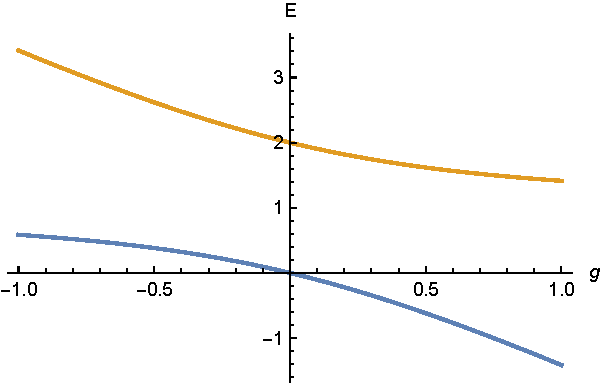
\includegraphics{sol2.pdf}
		\caption{Analytical eigenvalues for two particles and two levels ($\xi=1$)}
		\label{fig:2lev_analytical}
	\end{figure}

\section{Solution for four particles}

	For four particles and four holes (and no broken pairs), there are six available basis states. These are listed and labeled in Table~\ref{tab:4basis}.

	\begin{table}
		\centering
		\begin{tabular}{c c}
			\toprule
			Label & State \\
			\midrule
			\ket{1234} & \ket{1+1-2+2-} \\
			\ket{1256} & \ket{1+1-3+3-} \\
			\ket{1278} & \ket{1+1-4+4-} \\
			\ket{3456} & \ket{2+2-3+3-} \\
			\ket{3478} & \ket{2+2-4+4-} \\
			\ket{5678} & \ket{3+3-4+4-} \\
			\bottomrule
		\end{tabular}
		\caption{Basis states for four particles and four levels}
		\label{tab:4basis}
	\end{table}

	Acting on the states one-by-one, we find
	\begin{align*}
		\hat H \ket{1234} &= 2\xi\ket{1234} - g( 2\ket{1234} + \ket{1256} + \ket{1278} + \ket{5634} + \ket{7843}) \\
			&= 2\xi\ket{1234} - g( 2\ket{1234} + \ket{1256} + \ket{1278} + \ket{3456} + \ket{3478}) \\
		\hat H \ket{1256} &= 4\xi\ket{1256} - g(2\ket{1256} + \ket{1234} + \ket{1278} + \ket{3456} + \ket{7856})  \\
			&= 4\xi\ket{1256} - g(2\ket{1256} + \ket{1234} + \ket{1278} + \ket{3456} + \ket{5678}) 
	\end{align*}
	and so on. In other words, the diagonal elements (the expectation values) get a contribution from the single-particle energies, and any matrix element whose bra differs from its ket by at most one pair of single particle states gets a contribution of $-g$. The expection values also get a contribution of $-2g$ from the two-body operator since they can be formed by destroying and then re-creating either pair. Using this information, the Hamiltonian matrix can be written as:
	\begin{equation}
		\mathbf{H} = \begin{pmatrix}
			2\xi - 2g & -g & -g & -g & -g & 0  \\
			-g & 4\xi - 2g & -g & -g & 0  & -g \\
			-g & -g & 6\xi - 2g & 0  & -g & -g \\
			-g & -g &  0 & 6\xi - 2g & -g & -g \\
			-g &  0 & -g & -g & 8\xi - 2g & -g \\
			 0 & -g & -g & -g & -g & 10\xi - 2g\\
		\end{pmatrix}.
	\end{equation}
	There is no analytical solution for the eigenvalues of this matrix, but if we let $\xi=1$ and $g=0$, then the eigenvalues are $\{2, 4, 6, 6, 8, 10\}$, the single-particle energies. Fig.~\ref{fig:4lev_analytical} shows a plot of the eigenvalues as a function of $g$. Based on this, it appears that the ground state becomes bound for $g$ greater than about 0.65.

	\begin{figure}[p]
		\centering
		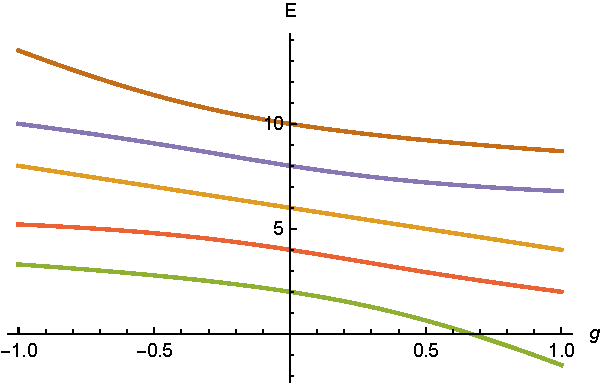
\includegraphics{sol4.pdf}
		\caption{Analytical eigenvalues for four particles and four levels ($\xi=1$)}
		\label{fig:4lev_analytical}
	\end{figure}

\section{Results from code}
	
	I wrote a small Python module to calculate the eigenvalues. It can be found in the GitHub repository \url{https://github.com/jbradt/structure_work/} in the directory \texttt{project/shellcode}. This program is perhaps not the fastest thing in the world, but it was written with simplicity in mind, and not efficiency.

	The program generates the single-particle states for the pairing model internally and then finds the possible Slater determinants. These are then used to find the Hamiltonian matrix, which can then be diagonalized. The interactions for the Hamiltonian are written directly into the code, which is not ideal, but is perhaps less inconvenient in Python than it would be in a compiled language. The usage of the code is documented in the docstrings of the source file itself.

	After running the code for the cases in the previous two parts, I created two graphs of the results for varying values of $g$. Fig.~\ref{fig:2lev_calc} shows the results for two particles and two levels, and Fig.~\ref{fig:4lev_calc} shows the results for four particles and four levels. These results look just like the analytical results from the previous parts.

	\begin{figure}[p]
		\centering
		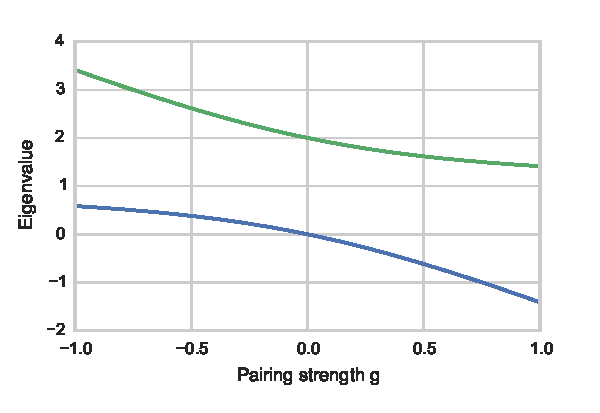
\includegraphics{calc2.pdf}
		\caption{Calculated eigenvalues for two particles and two levels ($\xi=1$)}
		\label{fig:2lev_calc}
	\end{figure}

	\begin{figure}[p]
		\centering
		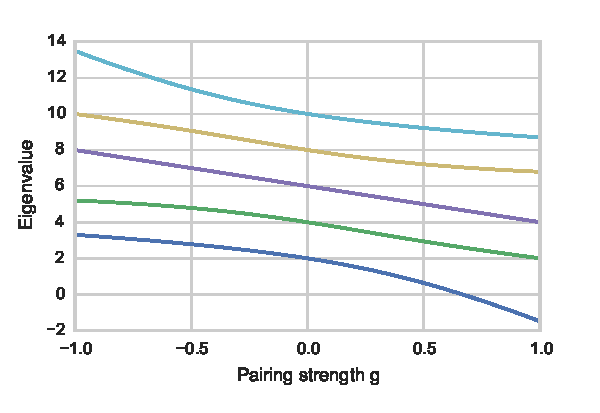
\includegraphics{calc4.pdf}
		\caption{Calculated eigenvalues for four particles and four levels ($\xi=1$)}
		\label{fig:4lev_calc}
	\end{figure}

\section{Further tests}

	One way to test the code is to remove the pairing interaction. This is equivalent to letting $g \rightarrow 0$. If I generate the Hamiltonian matrix for four particles and four levels, leaving the pairs-only restriction in place to make comparisons easy, I get the following matrix:
	\begin{equation*}
		\mathbf{H} = \begin{pmatrix}
			2 & 0 & 0 & 0 & 0 & 0  \\
			0 & 4 & 0 & 0 & 0 & 0  \\
			0 & 0 & 6 & 0 & 0 & 0  \\
			0 & 0 & 0 & 6 & 0 & 0  \\
			0 & 0 & 0 & 0 & 8 & 0  \\
			0 & 0 & 0 & 0 & 0 & 10 \\
		\end{pmatrix}.
	\end{equation*}
	This matrix is diagonal, so the eigenvalues are $\{2, 4, 6, 6, 8, 10\}$, which are just the single-particle energies, as expected.

	The code can also be tested by putting all of the particles into a single, highly degenerate energy level. According to the assignment, for a single state with degeneracy $\Omega = 2j+1$, the ground state energy is
	\begin{equation}
		E_0 = -\frac{g}{4} n (\Omega - n + 2)
	\end{equation}
	To test this, I calculated the Slater determinants for a single state with $p=1$ and $j=5/2$, which allows 6 particles to all fit into the ground state. I restricted the calculation to pairs of particles with opposite spin projections (e.g. 1/2 and -1/2). The results are compared for different values of $g$ in Fig.~\ref{fig:gs6}. I performed the same calculation for 8 particles in a state with $j=7/2$, and the results of that calculation are shown in Fig.~\ref{fig:gs8}. In both cases, the lines for the calculated and exact results overlap.

	\begin{figure}[p]
		\centering
		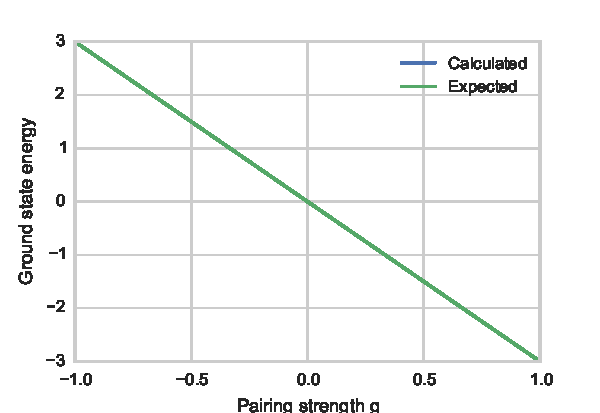
\includegraphics{gs6.pdf}
		\caption{Ground state energy as a function of $g$ for 6 particles in a 6-fold degenerate state}
		\label{fig:gs6}
	\end{figure}

	\begin{figure}[p]
		\centering
		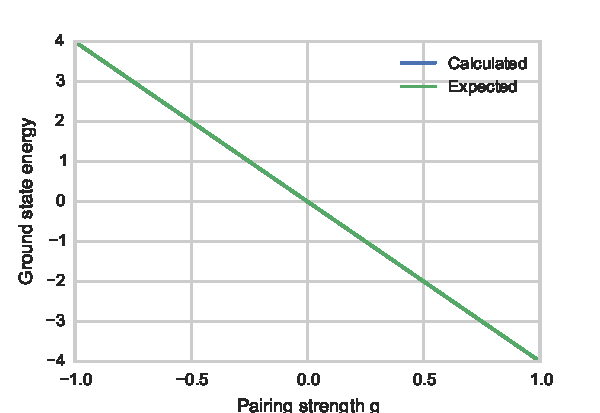
\includegraphics{gs8.pdf}
		\caption{Ground state energy as a function of $g$ for 8 particles in an 8-fold degenerate state}
		\label{fig:gs8}
	\end{figure}

	Finally, I ran the same sort of calculation as in the previous parts, except for 6 and 8 particles instead of 2 or 4. The results of this are shown in Fig.~\ref{fig:6lev_calc} and Fig.~\ref{fig:8lev_calc}. These follow the same general pattern as we saw for 2 and 4 particles.

	\begin{figure}[p]
		\centering
		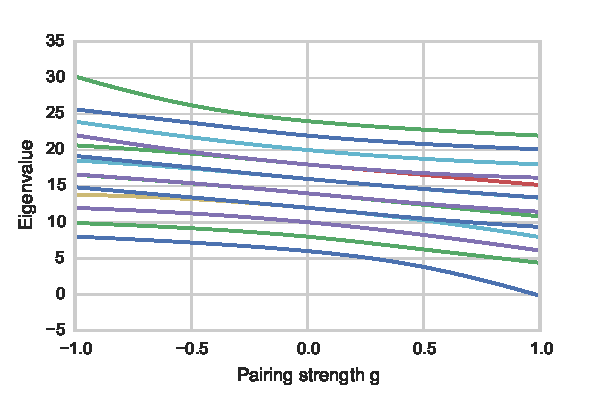
\includegraphics{calc6.pdf}
		\caption{Calculated eigenvalues for six particles and six levels ($\xi=1$)}
		\label{fig:6lev_calc}
	\end{figure}

	\begin{figure}[p]
		\centering
		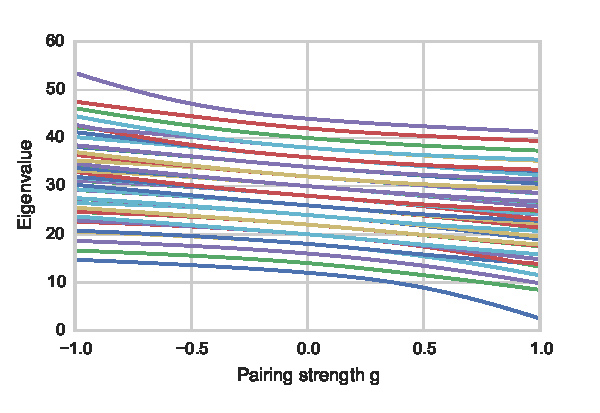
\includegraphics{calc8.pdf}
		\caption{Calculated eigenvalues for eight particles and eight levels ($\xi=1$)}
		\label{fig:8lev_calc}
	\end{figure}



\end{document}